\documentclass[border=3pt]{standalone}

\usepackage{tikz}
\usepackage[latin1]{inputenc}
\usetikzlibrary{positioning, arrows.meta, decorations.markings,calc}
\renewcommand{\familydefault}{\sfdefault}

\begin{document}
		
	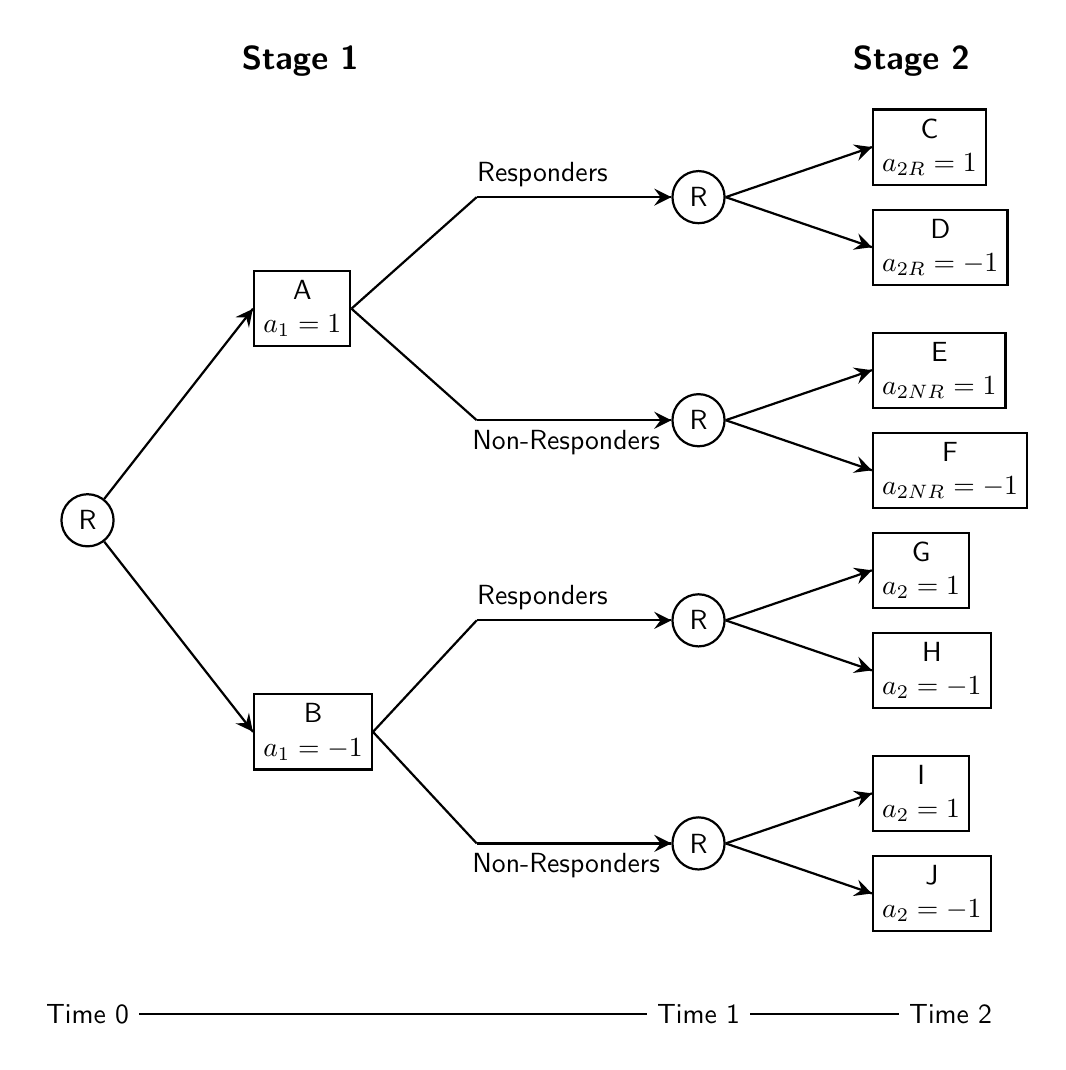
\begin{tikzpicture}[%
		node distance=6mm,
		randomize/.style={
			circle,
			minimum size=6mm,
			thick,
			black,
			draw
		},
		rerand/.style={
			xshift = 15mm
		},
		treatment/.style={
			rectangle,
			minimum size = 7mm,
			thick,
			black,
			anchor=west,
			align=center,
			draw
		},
		blank/.style={
			rectangle,
			minimum size=2mm
		},
		subgroup/.style={
			rectangle,
			rounded corners=1.5mm,
			thin,
			minimum size=6mm,
			black,
			draw
		},
		rlabel/.style={
%			font=\footnotesize,
			above,
			xshift=-4mm,
			align=left
		},
		nrlabel/.style={
%			font=\footnotesize,
			below,
			xshift=-1mm,
			align=left
		},
		trialarrow/.style={
			thick,
			decoration={markings,mark=at position 1 with  {\arrow[scale=1.5,>=stealth]{>}}},
			postaction={decorate}
		},
		subsetarrow/.style={
			thin,
			decoration={markings,mark=at position 1 with {\arrow[scale=1.2,>=stealth]{>}}},
			postaction={decorate}
		}, thick]
						
		\matrix[row sep=-2mm,column sep=12mm] { %
			& \node [align=center,xshift=6mm] {\large \textbf{Stage 1}}; & & & \node [align=center,xshift=5mm] {\large \textbf{Stage 2}}; \\[5mm]
			
			% DESIGN I
			
			& & & & \node (C-I) [treatment] {C \\ $a_{2R} = 1$};\\
			& & \node (b1-I) [blank] {}; & \node (R2-I) [randomize, rerand] {R}; & \\
			& & & & \node (D-I) [treatment] {D \\ $a_{2R} = -1$};\\
			& \node (A-I) [treatment] {A \\ $a_{1} = 1$}; & & & \\
			& & & & \node (E-I) [treatment] {E \\ $a_{2NR} = 1$}; \\
			& & \node (b2-I) [blank] {}; &s \node (R3-I) [randomize, rerand] {R}; & \\
			& & & & \node (F-I) [treatment] {F \\ $a_{2NR} = -1$}; \\
			\node (R1-I) [randomize] {R}; & & & &\\
			& & & & \node (G-I) [treatment] {G \\ $a_{2} = 1$}; \\
			& & \node (b3-I) [blank] {}; & \node (R4-I) [randomize, rerand] {R}; & \\
			& & & & \node (H-I) [treatment] {H \\ $a_{2} = -1$}; \\
			& \node (B-I) [treatment] {B \\ $a_{1} = -1$}; & & &\\
			& & & & \node (I-I) [treatment] {I \\ $a_{2} = 1$};\\
			& & \node (b4-I) [blank] {}; & \node (R5-I) [randomize, rerand] {R}; & \\
			& & & & \node (J-I) [treatment] {J \\ $a_{2} = -1$}; \\[1cm]
			
			% TIMEPOINTS
			
			\node (time0) [align=center, anchor=center] {Time 0};& & & \node (time1) [align=center, anchor=center, xshift=15mm] {Time 1}; & \node (time2) [align=center, xshift = 10mm] {Time 2}; \\
		};
	
%		\draw[dashed,lightgray] (time1.north) -- (R2-III.south);
%		\draw[dashed,lightgray] (R2-III.north) -- (R3-II.south);
%		\draw[dashed,lightgray] (R3-II.north) --++(90:3.2cm);
%		
%		\draw[dashed,lightgray] (time2.north west) --++(90:33cm);
	
		% DESIGN I LINES
	
		\draw[trialarrow] (R1-I) -- (A-I.west);
		\draw (A-I.east) -- (b1-I.center);
		\draw (A-I.east) -- (b2-I.center);
		\draw[trialarrow] (b1-I.center) -- node[rlabel] {Responders} (R2-I.west);
		\draw[trialarrow] (b2-I.center) -- node[nrlabel] {Non-Responders} (R3-I.west);
		\draw[trialarrow] (R2-I.east) -- (C-I.west);
		\draw[trialarrow] (R2-I.east) -- (D-I.west);
		\draw[trialarrow] (R3-I.east) -- (E-I.west);
		\draw[trialarrow] (R3-I.east) -- (F-I.west);
		
		\draw[trialarrow] (R1-I) -- (B-I.west);
		\draw (B-I.east) -- (b3-I.center);
		\draw (B-I.east) -- (b4-I.center);
		\draw[trialarrow] (b3-I.center) -- node[rlabel] {Responders} (R4-I.west);
		\draw[trialarrow] (b4-I.center) -- node[nrlabel] {Non-Responders} (R5-I.west);
		\draw[trialarrow] (R4-I.east) -- (G-I.west);
		\draw[trialarrow] (R4-I.east) -- (H-I.west);
		\draw[trialarrow] (R5-I.east) -- (I-I.west);
		\draw[trialarrow] (R5-I.east) -- (J-I.west);
		
		% TIME LINES
		
		\draw (time0) -- (time1) -- (time2);
\end{tikzpicture}
\end{document}